\documentclass[11pt,a4paper]{article}
\usepackage{gtu-el-yazisi}
\begin{document}
\notbilgi{Elektronik II}{Aktif yüklü fark yükselteci ve frekans cevabı}{Ders8.pdf}

\sayfa{1}
\begin{ornek}[7]
Consider the active loaded MOS differential amplifier with $(W/L)_n=100$, $(W/L)_p=\okunamadi{}$, $\mu_n C_{ox}=2\mu_p C_{ox}=0{,}2\ \mathrm{mA/V^2}$, $|V_A|_n=|V_A|_p=20\ \mathrm{V}$, $I=0{,}8\ \mathrm{mA}$, $R_{SS}=25\ \mathrm{k}\Omega$. Calculate $g_m$, $R_o$, $|A_d|$, $|A_c|$ and CMRR\footnote{Claude notu: Soru metni sayfa kenarında kesilmiş; ``loaded'', ``amplifier'', ``mA/V$^2$'' ve ``$|A_c|$'' tamamlanmıştır.}
\end{ornek}

\sekilnotu[1]{Aktif yüklü MOS fark yükselteci. Üstte $V_{DD}$ rayı; ona bağlı iki PMOS (3 ve 4 numaralı, ``Active load'' notlu, turuncu kesikli çerçeve içinde) akım aynası yükü: ortak gate hattı sol PMOS'un (3) drain düğümüne bağlı (diyot bağlı), sağ PMOS (4) çıkış düğümünü besliyor. Altta iki NMOS (1 solda, gate: $v_{G1}$; 2 sağda, gate: $v_{G2}$) fark çifti, turuncu kesikli çerçeve içinde. Sağ kolun (2 ve 4) birleştiği düğümden çıkış $v_O$ alınıyor. Her iki kolda aşağı doğru kırmızı ok ve ``0,4 mA''. Ortak source düğümü ile $-V_{SS}$ arasında $R_{SS}$ direnci ve ona paralel $I$ akım kaynağı (aşağı yönlü). Sol üstte daire içinde ``7''.}

\begin{cozum}
$g_{m1,2}=\ ?$ \qquad $\to\quad \dfrac{2(0{,}4)}{V_{OV}=0{,}2}=4\ \mathrm{mA/V}$

\[ 0{,}4=\tfrac12\cdot 0{,}2\cdot 100\,(V_{OV})^2 \qquad\Rightarrow\qquad 0{,}04=(V_{OV})^2 \ \Rightarrow\ V_{OV}=0{,}2 \]

$R_{SS}=25\ \mathrm{k}\Omega$

$r_{o\,1,2}=\dfrac{V_A}{I_D}=\dfrac{20}{0{,}4}=50\ \mathrm{k}\Omega$

$r_{o\,3,4}=r_{o\,1,2}=50\ \mathrm{k}\Omega$

\textit{differential mode}

\sekilnotu[1]{Fark modu yarım devresi: üstte $r_{o4}$ direnci (üst ucu sağa kısa bir çizgiyle AC toprağa/besleme hattına gidiyor), altında ``2'' numaralı NMOS'un drain'ine bağlı; gate'e $v_{id}/2$ uygulanmış; source toprağa bağlı.}

\begin{align*}
&= g_m\,(r_{o4}\parallel r_{o2}) \\
&= \tfrac12\, g_m r_o = \tfrac12\cdot 4\ \mathrm{mA/V}\cdot 50\ \mathrm{k}\Omega \\
&= 100\ [\mathrm{V/V}]
\end{align*}

\[ A_{cm}=\frac{1}{2\,g_m R_{SS}}=\frac{1}{2\times 4\ \mathrm{mS}\times 25\ \mathrm{k}\Omega}=\frac{1}{200} \]

\[ \mathrm{CMRR}=\frac{100}{\frac{1}{200}}=20\,000 \]

\[ 20\log\left(20\cdot 10^{3}\right)=86\ \mathrm{dB} \]
\end{cozum}

\section{Frequency response}
\sayfa{2}
\sekilnotu[2]{Yapıştırılmış basılı ders kitabı şekli: kazancın frekansla değişimi, $|V_o/V_{sig}|$ (dB) eksenine karşı $f$ (Hz, log ölçek). Alçak frekans bandı (``Gain falls off due to the effects of coupling and bypass capacitors''), orta bant (``All capacitances can be neglected'', $20\log|A_M|$ (dB), 3 dB düşüş) ve yüksek frekans bandı (``Gain falls off due to the internal capacitive effects of the BJT or the MOSFET''); alt ve üst kesim frekansları $f_L$ ve $f_H$.}

\sekilnotu[2]{Akım kaynağı ile kutuplanmış MOSFET ortak source yükselteç devresi (elle çizilmiş). Solda $v_{sig}$ kaynağı ve $R_{sig}$, ardından $C_{C1}$ kuplaj kondansatörü; gate düğümü $R_G$ ile toprağa bağlı. Drain üstte $R_D$ ile $V_{DD}$'ye bağlı; drain'den $C_{C2}$ kuplaj kondansatörü üzerinden $R_L$ yük direncine (toprağa) çıkış. Source'dan aşağı, $-V_{SS}$'e giden $I$ akım kaynağı ve ona paralel (toprağa bağlı) $C_S$ bypass kondansatörü. Turuncu kalemle üç bölge çevrilmiş: sol bölge ($v_{sig}$, $R_{sig}$, $C_{C1}$, $R_G$) ``due to $C_{C1}$''; sağ üst bölge ($R_D$, $C_{C2}$, $R_L$) ``due to $C_{C2}$''; alt bölge (akım kaynağı ve $C_S$) ``due to $C_S$''. Sol bölgeden kırmızı bir ok aşağıdaki ifadeye gidiyor.}

\[ \frac{1}{j\omega C} \]
\textit{(ifadenin altında kırmızı, kıvrımlı bir ok var)}

\sekilnotu[2]{Aynı devrenin ikinci çizimi; $C_{C1}$ kondansatörünün üzeri kırmızı kalemle işaretlenmiş (kondansatörün iki yanında kırmızı çift çizgi ve küçük oklar). Altında, kırmızı kalemle eşdeğer direnç şeması: soldaki uçtan $R_{sig}$ direnci, sağdaki uca bağlı $R_G$ direnci; iki uç arasında (kondansatörün olduğu yerde) çift yönlü ok ve altında ``$R_{eq}$''.}

\[ R_{eq}=R_{sig}+R_G \]

\[ \omega_{P1}=\frac{1}{C_{C1}\,(R_{sig}+R_G)} \]

\sayfa{3}
\section{2. kapasiteden kaynaklı etkiyi \texorpdfstring{\okunamadi{koyalım}}{koyalım}}
\sekilnotu[3]{Sol: MOSFET devresi (kapasitör etkisi için sadeleştirilmiş). Gate, ``$R$'' etiketli bir direnç üzerinden toprağa bağlı; drain, ``$R_D$'' direnciyle toprağa bağlı; source, ``$C_S$'' kondansatörü üzerinden toprağa bağlı. Sağ: küçük işaret eşdeğer devresi. Solda toprağa bağlı ``$R$'' direnci ve ``$+\,v_{gs}\,-$'' işaretli iki açık uç; alt hat (source düğümü) üzerine, toprağa bağlı bir test kaynağı $V_{tn}$ ve düğüme doğru yukarı yönlü $I_{tn}$ akımı bağlanmış; yanında bağımlı akım kaynağı $g_m v_{gs}$ ve paralelinde $r_o$ (kırmızı kalemle çizilerek iptal edilmiş, yanında kırmızı ``ihmal'') ile $R_D$.}

\[ \frac{V_{tn}}{I_{tn}} = \ ? \ = \frac{-v_{gs}}{-g_m\, v_{gs}} = \frac{1}{g_m} \]
\textit{(pay ve paydadaki $v_{gs}$ terimleri çizilerek sadeleştirilmiş)}

\[ \omega_{P2} = \frac{1}{\;\dfrac{C_S}{g_m}\;} = \frac{g_m}{C_S} \]

\sekilnotu[3]{Küçük işaret eşdeğer devresi: solda toprağa bağlı bir direnç ve iki açık uç (üstte gate, altta ``S'' düğümü); bağımlı akım kaynağı $g_m v_{gs}$; ``D'' düğümü ve ona bağlı $R_D$ (toprağa); ardından $C_{C2}$ kuplaj kondansatörü (iki ``L'' biçiminde çizilmiş, arada ok) ve toprağa bağlı $R_L$.}

\[ \omega_{P3} = \frac{1}{(R_D+R_L)\,C_{C2}} \]

\sekilnotu[3]{Yapıştırılmış basılı şekil: alçak frekans bölgesinde kazanç grafiği, $|V_o/V_{sig}|$ (dB) --- $f$ (Hz, log ölçek). Eğim $f_{P1}$'e kadar 60 dB/decade, $f_{P1}$--$f_{P3}$ arası 40 dB/decade, $f_{P3}$--$f_{P2}$ arası 20 dB/decade; $f_{P2}$'den sonra düz (orta bant, $20\log|A_M|$, $-3$ dB işareti, ``$\approx f_L$''). Kesikli düşey çizgiler $f_{P1}$, $f_{P3}$, $f_{P2}$'de.}

\noindent $\downarrow$ 2 pole, çünkü direnci yüksek

\noindent $\hookrightarrow$ dominant pole diğerlerinin \okunamadi{Ekatıkalan}

\sayfa{4}
\[ A_{mid} = -\left[\frac{R_G}{R_{sig}+R_G}\right] g_m\,(R_D \parallel R_L) \]

\[ A(s) = A_{mid}\left[\frac{s}{s+\omega_{P1}}\right]\left[\frac{s}{s+\omega_{P2}}\right]\left[\frac{s}{s+\omega_{P3}}\right] \]

\[ f_L = \frac{1}{2\pi}\left(\frac{1}{R_1 C_1}+\frac{1}{R_2 C_2}+\frac{1}{R_3 C_3}\right) \]

\begin{center}
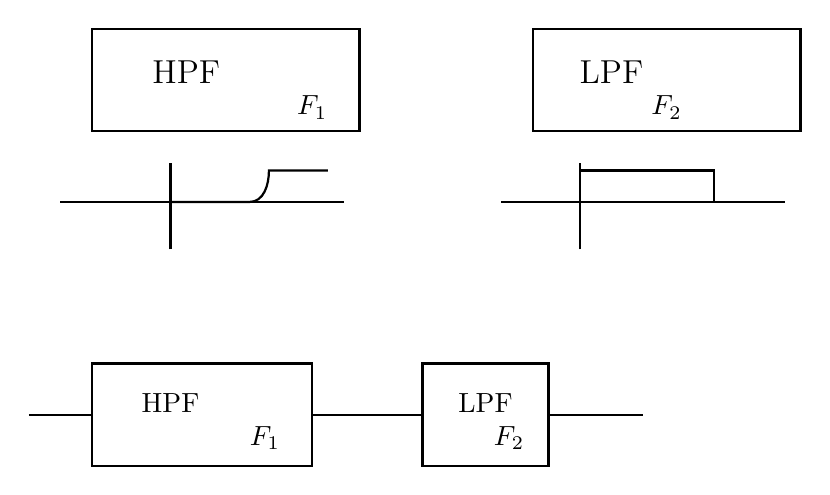
\begin{tikzpicture}[line width=0.8pt]
  % HPF kutusu ve cevabı
  \draw (0,0) rectangle (3.4,1.3); \node at (1.2,0.75) {\large HPF}; \node at (2.8,0.3) {$F_1$};
  \draw (-0.4,-0.9) -- (3.2,-0.9);
  \draw (1.0,-1.5) -- (1.0,-0.4);
  \draw (1.0,-0.9) -- (2.0,-0.9) to[out=0,in=-90] (2.25,-0.5) -- (3.0,-0.5);
  % LPF kutusu ve cevabı
  \begin{scope}[xshift=5.6cm]
    \draw (0,0) rectangle (3.4,1.3); \node at (1.0,0.75) {\large LPF}; \node at (1.7,0.3) {$F_2$};
    \draw (-0.4,-0.9) -- (3.2,-0.9);
    \draw (0.6,-1.5) -- (0.6,-0.4);
    \draw (0.6,-0.5) -- (2.3,-0.5) -- (2.3,-0.9);
  \end{scope}
  % seri bağlantı
  \begin{scope}[yshift=-3.6cm]
    \draw (-0.8,0) -- (0,0);
    \draw (0,-0.65) rectangle (2.8,0.65); \node at (1.0,0.15) {HPF}; \node at (2.2,-0.3) {$F_1$};
    \draw (2.8,0) -- (4.2,0);
    \draw (4.2,-0.65) rectangle (5.8,0.65); \node at (5.0,0.15) {LPF}; \node at (5.3,-0.3) {$F_2$};
    \draw (5.8,0) -- (7.0,0);
  \end{scope}
\end{tikzpicture}
\end{center}

\sekilnotu[4]{PNP BJT'li yükselteç devresi (emiter yukarıda). Üstte $V_{EE}$ (yukarı ok) ile beslenen, aşağı yönlü bir akım kaynağı emitere bağlı; emiter düğümü ayrıca $C_E$ bypass kondansatörü ile toprağa bağlı. Base: solda $v_{sig}$ kaynağı, $R_{sig}$ ve $C_{C1}$ kuplaj kondansatörü üzerinden base'e bağlı; base ayrıca $R_B$ ile toprağa bağlı. Kolektör: aşağıda $R_C$ üzerinden $V_{CC}$ kaynağına (aşağı ok) bağlı; kolektörden $C_{C2}$ kuplaj kondansatörü ile toprağa bağlı $R_L$ yük direncine ve $v_{out}$ çıkışına gidiyor.}

\[ A_m = -g_m\,(R_C \parallel R_L)\,\frac{(R_B \parallel r_\pi)}{R_{sig}+(R_B \parallel r_\pi)} \]

\begin{center}
\begin{circuitikz}[american]
  \draw (0,0) to[R=$R_{sig}$] (2.2,0) -- (4.8,0);
  \draw (2.8,0) to[R=$R_B$] (2.8,-1.9) node[ground]{};
  \draw (4.2,0) to[R=$r_\pi$] (4.2,-1.9) node[ground]{};
\end{circuitikz}
\end{center}

\[ A_m = -g_m\,(R_C \parallel R_L)\,\frac{(R_B \parallel r_\pi)}{R_{sig}+(R_B \parallel r_\pi)} \]

\sayfa{5}
\sekilnotu[5]{Küçük işaret eşdeğer devresi (BJT): solda toprağa bağlı uçtan $R_{sig}$, ardından $C_{C1}$ kondansatörü (çift çizgi, altında küçük bir ok işareti); sonraki düğümden toprağa $R_B$; aynı düğümden aşağı $r_\pi$, alt ucu kalın bir telle bağımlı akım kaynağı $g_m v_\pi$'nin alt ucuna bağlı; kaynağın üst ucundan giden hat toprağa bağlı $R_C$'ye gidiyor.}

\sekilnotu[5]{Aynı devre; $C_{C1}$ yerine seri bir test kaynağı $V_{tn}$ (daire içinde) konmuş, altında sağa doğru ok ve ``$I_{tn}$''. Diğer elemanlar aynı ($R_{sig}$, $R_B$, $r_\pi$, $g_m v_\pi$, $R_C$).}

\[ R_1 = R_{CC1} = \bigl(R_{sig} + (R_B \parallel r_\pi)\bigr) \]

\[ \omega_{P1} = \frac{1}{C_{C1}\,\bigl(R_{sig} + (R_B \parallel r_\pi)\bigr)} \]

\noindent $C_E$ den bakarken

\noindent Low frekansta C'ler short kabul edilir

\sekilnotu[5]{Soldan toprağa bağlı uçtan $R_{sig}$; sonraki düğümden toprağa $R_B$; sağdaki düğüm ``B'' olarak işaretli; ``B''den aşağı $r_\pi$; $r_\pi$'nin alt ucundan sağa bir hat ve hattın ucunda toprağa bağlı bir kondansatör, yanında ``$R_{out}$'' etiketi.}

\[ R_{CE} = R_2 = \frac{(R_{sig} \parallel R_B) + r_\pi}{\beta + 1} \]

\[ \omega_{P2} = \frac{1}{\dfrac{(R_{sig} \parallel R_B) + r_\pi}{\beta + 1}\; C_E} \]

\[ \omega_{P3} = \frac{1}{C_{C2}\,(R_C + R_L)} \]

\end{document}
